% \documentclass[11pt,reqno,draft]{amsart}
\documentclass[11pt,reqno]{amsart}
%% Escrevendo em português:
\usepackage[brazil]{babel}
%\usepackage[T1]{fontenc}
\usepackage{lmodern}
%----------------------------

%----------------------------
%\documentclass[11pt,reqno]{amsart}
\usepackage[utf8x]{inputenc}
\usepackage{amsfonts}
\usepackage{amsmath,calc} %para usar ocm LPs
\usepackage{mathtools,amssymb} %para usar com LPs
\usepackage{amsthm}
\usepackage{subfigure}
\usepackage[toc,page]{appendix}
%\usepackage[subnum]{cases} %numerar
\usepackage{cases} %numerar

\usepackage{siunitx}

%LP formulation
\usepackage{lpform} %LPs
\renewcommand{\lpforall}[1]{&& \forall #1}

\newcommand{\dist}{{\rm dist}}

%reset equation number whenever section and subsection is stepped
\usepackage{chngcntr}
\counterwithin*{equation}{section}
\counterwithin*{equation}{subsection}

%meus ambientes
\newtheorem{definicao}{Definição}
\newtheorem{notacao}{Notação}
%\newtheorem{teorema}{Teorema}[section]
\newtheorem{teorema}{Teorema}
\newtheorem{proposition}{Proposition}
\newtheorem{afirmacao}{Afirmação}[teorema]
%\newtheorem{lema}{Lema}[section]
\newtheorem{lema}{Lemma}
\newtheorem{observacao}{Observação}
%\newtheorem{proposicao}{Proposição}[section]
\newtheorem{proposicao}{Proposição}
%\newtheorem{corolario}{Corolário}[section]
\newtheorem{corolario}{Corolário}
\newtheorem{conjectura}{Conjectura}
\newtheorem{problema}{Problema}
\newtheorem{exemplo}{Exemplo}

\newcommand{\incid}{\mathcal{X}}

\title{MMST}
\author{Hugo Braga}
\date{2015}

\begin{document}

\maketitle

\section{Introdução}
Neste texto, a menos de menção em contrário, os grafos considerados
são não-orientados, simples e conexos.  Dado um grafo $G=(V,E)$, 
uma função custo $w: E \to \mathbb{R}^+$ e um
real $t \ge 1$, chamado de \emph{fator de dilatação}, um
\emph{$t$-spanner} é um subgrafo gerador $H$ de $G$ tal que:
\begin{equation}
%\label{eq:spanner}
\dist_{H}(u,v) \le t \cdot \dist_{G}(u,v), \quad \forall\;u,v \in V, 
\label{eq:def_spanner}
\end{equation}

\noindent onde $\dist_{G}(u,v)$ denota a distância entre $u$ e $v$ em
$G$. A distância entre $u$ e $v$ em $G$ é calculada através do 
somatório do custo (definido pela 
função $w$) das arestas de um caminho de custo mínimo entre $u$ e $v$ em $G$. 
Quando $H$ é uma árvore dizemos que $H$ é uma \emph{árvore $t$-spanner}. 
Seja $(\incid^{H})_{e \in E(G)}$ o vetor de incidência de $H$.
Para $u,v \in V(H)$, seja $H_{u,v}$ o caminho entre $u$ e $v$ na árvore  $H$.
Além disso, para um grafo $G$, considere $V(G)$ o conjunto 
dos vértices de $G$ e $E(G)$ o conjunto das arestas de $G$.

Cai e Corneil \cite{CaiC1995} 
mostraram que várias definições de t-spanner são equivalentes. 
Seja $Q$ um subgrafo gerador conexo de $G$.
Dentre as definições que são equivalentes com (\ref{eq:def_spanner}), estão:

\begin{equation}
\dist_{Q}(u,v) \le t \cdot \dist_{G}(u,v), \quad \forall\;uv \in E(G).
\label{eq:def2_spanner}
\end{equation}

A prova de que (\ref{eq:def_spanner}) implica em (\ref{eq:def2_spanner}) 
é direta. 
Vamos provar que (\ref{eq:def2_spanner}) implica em (\ref{eq:def_spanner}). 

\begin{observacao}
\label{obs:relate_spanner_definitions}
Seja $Q$ um subgrafo gerador conexo de $G$. Então
\begin{equation*}
\begin{split}
\dist_{Q}(u,v) \le t \cdot \dist_{G}(u,v), \forall\;uv \in E(G) \implies \\
\dist_{Q}(u,v) \le t \cdot \dist_{G}(u,v), \forall\;u,v \in V(G).
\end{split}
\end{equation*}
\begin{proof}
Seja $u,v \in V(G)$. Se $uv \in E(G)$, por hipótese, segue a conclusão. 
Vamos assumir que $uv \notin E(G)$. Seja 
$P = (u = u_0, u_1, ..., u_{l-1}, u_l = v)$ um caminho de custo mínimo entre 
$u$ e $v$ em $G$. Por hipótese, para cada \\
\mbox{$u_{i-1}u_i \in E(P), \dist_{Q}(u_{i-1},u_i) \le t \cdot \dist_{G}(u_{i-1},u_i)$}.
 Então: 
\begin{align*}
\dist_{Q}(u,v) &= \sum_{i = 1}^{l} dist_{Q}(u_{i-1},u_i)\\ 
&\le \sum_{i = 1}^{l}t \cdot \dist_{G}(u_{i-1},u_i)\\
&= t \cdot \sum_{i = 1}^{l} \dist_{G}(u_{i-1},u_i)\\
&= t \cdot \dist_{G}(u,v),
\end{align*}
onde a primeira e última igualdade seguem do fato de que o custo de um 
caminho mínimo é igual ao somatório do custo das arestas que compoem o 
caminho mínimo.
\end{proof}
\end{observacao}

Uma versão de otimização para o problema árvore \hbox{$t$-spanner}
corresponde em minimizar o fator de dilatação. Formalmente, o problema
é definido como: dado um grafo $G=(V,E)$ e uma 
função custo $w: E \to \mathbb{R}^+$, o \emph{problema de árvore spanner mínima}
(\emph{Minimum Max-Stretch Spanning Tree} - MMST) tem por objetivo
encontrar o menor~$t$ (real) tal que $G$ admite uma árvore
$t$-spanner. 

\section{Formulação}
Considere a variável de decisão $x \in \{0,1\}^{E}$ com o seguinte 
significado: $x(e), e \in E$, é igual a 1 se e somente se $e$ faz parte da 
solução e 0 caso contrário. Considere a variável de decisão 
$Y \in \{0,1\}^{E \times E}$ com o seguinte significado: 
para $e = uv,f \in E(G)$, se $f$ faz parte do caminho entre $u$ e $v$ na 
solução então $Y(e,f) = 1$. Se $Y$ possui suporte mínimo, então o lado oposto 
da implicação também vale. 
% $Y(e,f), e,f \in E$, 
% é igual a 1 se e somente se para $e = uv$, $f$ faz parte do caminho entre 
% $u$ e $v$ na solução e 0 caso contrário.

A seguir, apresentamos uma modelagem para o MMST. Para $e \in E(G)$, 
considere $\delta(S)$ como sendo o conjunto de arestas que tem 
exatamente um dos vértices em $S$. 
%tal que $e$ faz parte deste conjunto de arestas.

\begin{lpformulation}[(P)]
\lpobj*{min}{t}
\lpeq[res_mmst:path]{Y(e,\delta(S)) \ge 1}{e \in E, \forall S \subset V, |S \cap e| = 1}
\lpeq[res_mmst:tree]{x(E) = |V| - 1}{}
\lpeq[res_mmst:relate_vars]{Y(e,f) \le x(f)}{e,f \in E}
\lpeq[res_mmst:spanner]{\sum_{f \in E}Y(e,f) w(f) \le 
%\lpnewline\qquad\qquad 
t \cdot \dist_{G}(u,v)}{e=uv \in E}
\lpeq[res_mmst:t]{t \ge 1}{}
\lpeq[res_mmst:int_x]{x(e) \in \{0,1\}}{e \in E}
\lpeq[res_mmst:int_Y]{Y(e,f) \in \{0,1\}}{e,f \in E}
\lpeq[res_mmst:real_t]{t \in \mathbb{R}^+}{}
\lplabel{lp:primal_mmst}
\end{lpformulation}
% onde $\delta(S)$ corresponde ao conjunto de arestas que tem exatamente 
% um dos vértices em $S$.

\begin{afirmacao}
\label{afirm:sol_viavel_lp}
Para uma árvore $t'$-spanner $T$ de um grafo $G$, existe 
uma solução viável $Sol = (x', Y', t')$ de \ref{lp:primal_mmst}. 
Ademais, $Y'$ possui suporte mínimo.
\begin{proof}
Para cada $e = uv, f \in E(G)$, 
podemos construir uma solução viável $Sol = (x', Y', t')$ de 
\ref{lp:primal_mmst} a partir de $(T,t')$ da seguinte forma:

\begin{align}
x'(e) \leftarrow \incid^{T}_{e},\quad\quad\quad\quad\quad\quad\quad\quad\quad\quad\quad\quad\quad\quad\quad\quad\quad\quad\quad\quad\;\label{regra:1}
\end{align}
\begin{subnumcases}{Y'(e,f)\leftarrow}
    1& \text{se $e \in E(T), f = e,$}\\
    0& \text{se $e \in E(T), f \neq e,$}\label{regra:2b}\\
    1& \text{se $e \in  E(G) \setminus E(T), f \in E(T_{u,v}),$}\\
    0& \text{se $e \in  E(G) \setminus E(T), f \in E(G) \setminus E(T_{u,v}).$}
\end{subnumcases}

Seja $e = uv \in E(G)$ e $f = xy \in E(T)$ tal que $Y'(e,f) = 1$. Note que 
$f \in E(T_{u,v})$. Seja 
$T_{u,v} = \{u = u_0, u_1, ., u_i = x, u_{i+1} = y, ..,  u_{l-1}, u_l = v\}$. 
Caso $Y'(e,f) \leftarrow 0$, para $S = \{u_0, u_1, .., u_i\}$ e a aresta $f$, 
a restrição \ref{res_mmst:path} é violada. Segue que $Y'$ tem suporte mínimo.
\end{proof}
\end{afirmacao}

Vamos agora provar o sentido inverso. Vamos mostrar que uma solução viável de 
\ref{lp:primal_mmst} corresponde a uma solução viável do MMST. 
Seja $Sol = (x',Y',t')$ uma solução viável de \ref{lp:primal_mmst} 
tal que $Y'$ tem suporte mínimo. 
Para $e \in E$, seja $F(e) = \{f \in E: Y'(e,f) = 1\}$. 
Seja $G' = G[\bigcup_{e \in E}F(e)]$. 
Seja $E_{x} = \{e \in E: x'(e) = 1\}$. Seja $H = G[E_{x}]$.

A restrição \ref{res_mmst:path}
%é oriunda do trabalho de Goemans e Williamson \cite{GoemansW1995} e 
serve para garantir que $G'$ seja um subgrafo gerador conexo de $G$. A 
seguir, provaremos tal propriedade.

\begin{proposicao}
\label{prop:Yuv_caminho}
Para cada $e = uv \in E(G)$, existe um caminho entre $u$ e $v$ em 
$G[F(e)]$.
\begin{proof}
Seja $e = uv \in E(G)$. Suponha (por absurdo) que não existe um 
caminho entre $u$ e $v$ em $G[F(e)]$. Então $u$ e $v$ estão 
em componentes distintas em $G[F(e)]$. Seja $G_u$ o grafo induzido pelos 
vértices do componente de $G[F(e)]$ que contém $u$. Seja $S = V(G_u)$. Mas 
então a restrição \ref{res_mmst:path} é violada para $S$ e $e$, 
contradizendo a hipótese de que $Sol$ é uma solução 
viável de \ref{lp:primal_mmst}.
\end{proof}
\end{proposicao}

\begin{proposicao}
\label{prop:gerador_conexo_G}
%Para todo $uv \in E$, existe um caminho entre $u$ e $v$ em $G'$.
O subgrafo $G'$ é gerador conexo de $G$.
\begin{proof}
Seja $u,v \in V(G)$. Como $G$ é conexo, existe um caminho 
$P = (u = u_0, u_1, ..., u_{l-1}, u_l = v)$ entre $u$ e $v$ em $G$. 
Pela proposição \ref{prop:Yuv_caminho} e sabendo que $G[F(e)] \subseteq G'$, 
para cada $u_{i-i}u_{i} \in E(P)$, existe um caminho entre $u_{i-1}$ e 
$u_{i}$ em $G'$. 
Sendo assim, $u$ e $v$ estão conectados em $G'$. Segue que $G'$ é um 
subgrafo gerador conexo de $G$.
\end{proof}
\end{proposicao}

A restrição \ref{res_mmst:tree} assim como a restrição 
\ref{res_mmst:relate_vars} é necessária para garantir que a solução seja  
uma árvore. De maneira mais geral, a restrição \ref{res_mmst:relate_vars} 
diz que para $f \in E(G)$, se $Y(e,f) = 1$ para algum $e \in E(G)$, então $f$ 
deve fazer parte da solução final. Além disso, se $f \in E(G)$ 
não faz parte da solução final, não existe $e \in E(G)$ tal que $Y(e,f) = 1$. 
Em outras palavras, $E(G') \subseteq E(H)$.

\begin{proposicao}
\label{prop:x_arvore}
$H$ é uma árvore geradora de $G$.
\begin{proof}
Em decorrência da proposição \ref{prop:gerador_conexo_G} e da restrição 
\ref{res_mmst:relate_vars}, para cada $u,v \in V(G)$, $H$ contém um caminho 
entre $u$ e $v$. Este fato juntamente com a restrição \ref{res_mmst:tree} 
implica que $E_{x}$ induz uma árvore geradora.
\end{proof}
\end{proposicao}

\begin{proposicao}
\label{prop:GY_arvore}
$G' = H$.% é uma árvore geradora de $G$.
\begin{proof}
Segue da proposicao \ref{prop:gerador_conexo_G} juntamente com a proposição 
\ref{prop:x_arvore} e do fato de que $E(G') \subseteq E(H)$ (restrição 
\ref{res_mmst:relate_vars}).
\end{proof}
\end{proposicao}

Note que \ref{lp:primal_mmst} não possui uma variável associada aos 
caminhos que respeitam a restrição de spanner, como na modelagem tradicional 
\cite{SigurdZ2004,DinitzK2011}. 
%Seja $p, q \in V$.
Para verificar se um caminho 
a ser encontrado entre um par de vértices $u,v \in V(G)$ 
respeita esta restrição, $e=uv \in E(G)$, 
nós definimos uma variável específica $Y(e,f), \forall f \in E$, para o par 
de vértices $u,v$. 
O corolário a seguir é fundamental para entender por quê a restrição 
\ref{res_mmst:spanner} modela corretamente a restrição de spanner. Em seguida, 
provaremos que uma solução de \ref{lp:primal_mmst} 
respeita esta restrição.
% somamos o peso das 
% arestas que fazem parte do único 
% caminho existente em $G_{Y'}$ 
% entre $u$ e $v$ (corolário \ref{corol:GY_arvore}). Este caminho único é induzido 
% por $Y'(e,E)$ (corolário \ref{corol:Yuv_define_caminho}).  
% Para relacionar a 
% distância entre 
% $u$ e $v$ com o caminho existente entre $u$ e $v$ em 
% $G_{Y'}$ (lembrando que $G_{Y'} = H$), é necessário definir uma variável 
% específica $Y(e,f)$, para todo $f \in E$. 
% Isso decorre do fato da mesma 
% aresta poder fazer parte de caminhos entre pares diferentes de vértices. 
% Provaremos a seguir que uma solução de \ref{lp:primal_mmst} 
% (através da restrição \ref{res_mmst:spanner}) respeita a restrição de spanner.

\begin{corolario}
\label{corol:Yuv_define_caminho}
% Seja $Sol = (x', Y', t')$ uma solução viável de \ref{lp:primal_mmst} tal que 
% $Y'$ possui suporte mínimo. Então, 
Para cada $e = uv \in E$, $G[F(e)]$ é um 
caminho entre $u$ e $v$.
\begin{proof}
Seja $e = uv \in E(G)$. Pela proposição \ref{prop:Yuv_caminho}, existe um 
caminho $P$ entre $u$ e $v$ em $G[F(e)]$. Suponha (por absurdo) que existe 
$f = pq \in F(e)$ tal que $Y'(e,f) = 1$ e $f \notin E(P)$. Para cada 
$g,h \in E(H)$, seja $Y^* \in \{0,1\}^{E \times E}$ definido da seguinte forma: 
\begin{align*}
&Y^*(g,h)\leftarrow
\begin{cases}
    0& \text{se $g = e, h = f,$}\\
    Y'(g,h)& \text{caso contrário.}
\end{cases}
\end{align*}

Observe que as restrições 
\ref{res_mmst:path},\ref{res_mmst:relate_vars}, \ref{res_mmst:spanner} e 
\ref{res_mmst:int_Y} continuam sendo satisfeitas. 
Então, $Sol' = (x', Y^*, t')$
 é uma solução viável de \ref{lp:primal_mmst} tal que $Y^*$ possui um suporte 
menor do que $Y'$, uma contradição.
\end{proof}
\end{corolario}

\begin{proposicao}
\label{prop:x_spanner}
Para cada $uv \in E,\;\dist_{H}(u,v) \le t \cdot \dist_{G}(u,v)$.
\begin{proof}
Seja $e=uv \in E$.
Como vale o corolário 
\ref{corol:Yuv_define_caminho}, então \\
\mbox{$\dist_{G[F(e)]}(u,v) = \sum_{f \in E}Y'(e,f)\;w(f)$}. 
Como $G[F(e)] \subseteq G'$ e $G'$ é uma árvore 
(proposição \ref{prop:GY_arvore}), então 
\mbox{$\dist_{G'}(u,v) = \dist_{G[F(e)]}(u,v)$}. Como $H = G'$ (proposição 
\ref{prop:GY_arvore}) e $Sol$ respeita a restrição \ref{res_mmst:spanner}, 
segue que \\
$\dist_{H}(u,v) = \dist_{G'}(u,v) = \dist_{G[F(e)]}(u,v) = \sum_{f \in E} Y'(e,f) \; w(f) \le t \cdot \sum_{f \in E}Y'(e,f)\;w(f)$.
\end{proof}
\end{proposicao}

\begin{corolario}
\label{corol:standard_spanner}
Para todo $u,v \in V,\;\dist_{H}(u,v) \le t \cdot \dist_{G}(u,v)$.
\begin{proof}
Segue da proposição \ref{prop:x_spanner} e da observação 
\ref{obs:relate_spanner_definitions}.
\end{proof}
\end{corolario}

\begin{figure}[t] 
\centering
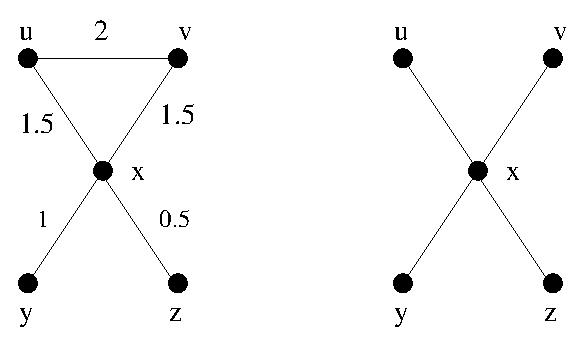
\includegraphics[scale=0.45]{figuras/exemplo_Y_minimal}
\caption{Um grafo com sua respectiva árvore t-spanner ótima}
\label{fig:exemplo_Y_minimal}
\end{figure}


No corolário \ref{corol:Yuv_define_caminho}, para $e = uv \in E(G)$, 
para mostrar que $G[F(e)]$ 
é um caminho entre $u$ e $v$, nós assumimos como hipótese que $Y'$ possui 
suporte mínimo. Esta hipótese não é condição necessária para que uma solução 
seja ótima.
Considere a figura \ref{fig:exemplo_Y_minimal}. Seja $G$ o grafo do lado 
esquerdo da figura. Observe que a árvore spanner ótima de $G$ corresponde à 
árvore no lado direito, cujo fator de dilatação $t^*$ é $1.5$. Seja 
$T$ esta árvore. Vamos 
construir uma solução viável $Sol^* = (x^*,Y^*,t^*)$ de \ref{lp:primal_mmst} 
aplicando a construção apresentada na afirmação \ref{afirm:sol_viavel_lp}, 
definida pelas atribuições \ref{regra:1} e 10, 
substituindo a atribuição \ref{regra:2b} pela seguinte atribuição:
\begin{align*}
&Y^*(e,f)\leftarrow
\begin{cases}
    1& \text{se $e = xy, f = xz, e \in E(T), f \neq e,$}\\
    0& \text{se $e \neq xy$ ou $f \neq xz, e \in E(T), f \neq e.$}
\end{cases}
\end{align*}
É fácil verificar que $Sol^*$ é uma solução viável de \ref{lp:primal_mmst} 
tal que $Y^*$ não tem suporte mínimo.

% Apesar de não ser uma condição necessária, para uma solução viável (ótima) 
% $(T^*,t^*)$ do 
% MMST, sabemos que existe uma solução viável (ótima) 
% $Sol^* = (x^*, Y^*, t^*)$ de 
% \ref{lp:primal_mmst} tal que $Y^*$ tem suporte mínimo (afirmação 
% \ref{afirm:sol_viavel_lp}). Sendo assim, a hipótese adotada no corolário 
% \ref{corol:Yuv_define_caminho} é válida.

\begin{afirmacao}
Uma solução viável de \ref{lp:primal_mmst} corresponde a uma solução viável 
do MMST.
\begin{proof}
Segue do fato da solução do PL ser uma árvore (proposição 
\ref{prop:x_arvore}), além do fato dos caminhos respeitarem a restrição 
de spanner (corolário \ref{corol:standard_spanner}). 
%e do $t$ ser minimizado na função objetivo.
\end{proof}
\end{afirmacao}

\section{Separação}

Na relaxação da formulação \ref{lp:primal_mmst}, o número de restrições do 
tipo \ref{res_mmst:path}, as quais denominaremos de 
\emph{inequações de corte}, é exponencial no tamanho de $V(G)$. 
Para tratar 
as restrições de tamanho exponencial, precisamos resolver o problema da 
separação. No problema da separação, dado um conjunto de restrições e uma 
(possível) solução, nós queremos saber se existe uma restrição que viola a 
solução. 
Em outras palavras, desejamos saber se a solução é viável ou obter um 
certificado que corresponda a uma restrição violada. 
%mostra que a solução é viável ou exiba uma restrição violada.

A separação das inequações de corte na relaxação de \ref{lp:primal_mmst} 
pode ser feita em tempo polinomial. Seja $(x^*, Y^*, t^*)$ uma solução 
da relaxação de \ref{lp:primal_mmst}. 
%Podemos interpretar a restrição \ref{res_mmst:path} da seguinte forma: 
Para cada $e=uv \in E(G)$, seja $G_{e} = (V, E')$, onde 
$E' = E(G)$ e $\forall_{f \in E'}w(f) \leftarrow Y^*(e,f)$. A capacidade de 
um $(u,v)$-corte mínimo em $G_{e}$ deve ser maior ou igual a $1$. Caso 
exista 
um $e=uv \in E(G)$ tal que um $(u,v)$-corte mínimo $\delta(W)$ em $G_{e}$ 
tenha valor menor do que $1$, então o par $(e,W)$ é um certificado de que a 
restrição \ref{res_mmst:path} é violada. Em decorrência do fato de que 
o valor de um $(u,v)$-fluxo máximo é igual à capacidade de um 
$(u,v)$-corte mínimo \cite{DantzigF1956}, existe um algoritmo de 
separação para as inequações de corte cuja complexidade 
computacional é $O(|E(G)|^{2} \cdot |V(G)|^{2})$ (teorema 8.30 em 
\cite{KorteV2012}).

 \bibliographystyle{amsplain}

 \bibliography{mmst}

\end{document}
